%\documentclass[11pt]{article}
%\usepackage{graphicx}
%\usepackage{amssymb, amsmath}
%\usepackage{bm}
%\usepackage{epstopdf}
%\DeclareGraphicsRule{.tif}{png}{.png}{`convert #1 `dirname #1`/`basename #1 .tif`.png}
%\usepackage{natbib}
%\usepackage{booktabs}
%%%%%%%%%%%%%%%%%%%%%%%%%%%%%%%%%%%%%%%%%%%%%%%%

%% To submit your paper:
\documentclass[draft,linenumbers]{agujournal}
%\draftfalse

%% For final version.
% \documentclass{agujournal}

\journalname{Global Biochemical Cycles}

\usepackage{bm}
\usepackage{booktabs}
\usepackage{amssymb, amsmath}
\usepackage{url}

\begin{document}


\title{Soil organic matter persistence as a stochastic process: age and transit time distributions of carbon in soils}

\authors{Carlos A. Sierra\affil{1}, Alison M. Hoyt\affil{1}, Yujie He\affil{2}, Susan E. Trumbore\affil{1}}


% \affiliation{1}{First Affiliation}
% \affiliation{2}{Second Affiliation}
% \affiliation{3}{Third Affiliation}
% \affiliation{4}{Fourth Affiliation}

\affiliation{1}{Max Planck Institute for Biogeochemistry, Hans-Kn\"oll-Str. 10, 07745 Jena, Germany}
\affiliation{2}{Department of Earth System Science, University of California, Irvine, USA}
%(repeat as many times as is necessary)

\correspondingauthor{C.A. Sierra}{csierra@bgc-jena.mpg.de}

%% Keypoints, final entry on title page.

% Example:
% \begin{keypoints}
% \item	List up to three key points (at least one is required)
% \item	Key Points summarize the main points and conclusions of the article
% \item	Each must be 100 characters or less with no special characters or punctuation
% \end{keypoints}


\begin{abstract}
The question of why some organic matter is more persistent than other that decomposes quickly in soils has motivated a large amount of research in recent years. Persistence is commonly characterized as turnover or mean residence time of soil organic matter (SOM). However, turnover and residence times are ambiguous measures of persistence,
because they could either represent the concepts of age or transit time.
To disambiguate these concepts and propose a metric to assess SOM persistence, we calculated age and transit time distributions for a wide range of soil organic carbon (SOC) models.
Furthermore, we show how age and transit time distributions can be obtained from a stochastic approach that takes a deterministic model of mass transfers among different pools and creates an equivalent stochastic model at the level of atoms.
Using this approach we show: 1) age distributions have relatively old mean values and long tails in relation to transit time distributions, suggesting that carbon stored in soils is on average much older than carbon in the release flux. 2) The difference between mean ages and mean transit times is large, with estimates of SOC persistence in the order of centuries or millennia when assessed using ages, and in the order of decades when using transit or turnover times. 3) The age distribution is an appropriate metric to characterize persistence of SOM.  An important implication of our analysis is that random chance is a factor that helps to explain why some organic matter persists for millennia in soil.  
\end{abstract}

\section{Introduction}
The observation that soil organic matter (SOM) persists in soils for a wide range of times independent of its quality has challenged previous views in SOM cycling research \citep{Kleber2010, Schmidt2011, Dungait2012, Gleixner2013, Paul2016}. It has been reported that easily degradable compounds can persist for years to decades in soils \citep{Kiem2003, Kleber2010}, while highly aromatic organic compounds such as lignin or charcoal can degrade in a matter of years, much faster than previously believed \citep{Gleixner1999, Kleber2010, Heim2007, Lehmann2015}. %Alternatively, the ages of SOM can also be much older, suggesting that some C persists in soils for centuries to millennia. 
To explain this variability, current research on mechanisms of SOM cycling and stabilization focus on physical and chemical protection rather than molecular structure to explain SOM persistence \citep{Schmidt2011, LehmannKleber}. 

The term persistence however, has been vaguely defined. In most cases, persistence is associated with the turnover or mean residence time of carbon in SOM \citep{Schmidt2011, Derrien2011, Lehmann2015}. These two terms are problematic to use as definitions of persistence for three main reasons: 1) they are ambiguously used in many studies, in some cases referring to the concept of age and in others to the concept of transit times (see below), 2) in some cases their calculation relies on the assumption of a single homogenous pool at steady-state while a range of timescales for C has been clearly reported \citep{Trumbore2000, Trumbore2009}, and 3) measures of central tendency do not provide information on the distribution of the maximum age that could be observed in a soil (Figure \ref{fig:example}). This highlights the need for a more precise definition of SOM persistence. %Here we evaluate soil age and transit time distributions in the context of SOM persistence.

Turnover and residence times are ambiguous terms because they may indicate concepts related to the age of carbon within the soil system or the age of carbon in the flux out of soils (e.g. CO$_2$ respiration or dissolved organic carbon leaching) \citep{Sierra2017}. Less ambiguous are the concepts of system age and transit times \citep{Bolin1973, Bruun2004, Derrien2011, Manzoni2009, Sierra2017}. System age can be defined as the age of particles or atoms in a system, in this case a soil, since the time the atom entered the system until the time of observation. Transit time can be defined as the time elapsed since the atom entered until it leaves in the output flux. It is well established that both system age and transit time are equal in single-pool systems at steady-state. For systems with multiple pools that cycle at different time scales, these quantities are generally different. 
 
System age and transit time can be characterized by a distribution that measures the proportion of atoms or particles in a soil that have less than a certain age \citep{Eriksson1971, Bolin1973}. These distributions can also be interpreted in a probabilistic sense, suggesting that the problem of persistence could also be approached from a stochastic point of view. 

In this manuscript, we assess age and transit time distributions to determine which is most appropriate to characterize the persistence of SOM. We focus on carbon cycling, but the ideas and theory presented can be applied to any other biogeochemical element \citep{Spohn2018}. To evaluate the applicability of these distributions, we calculate estimates of ages and transit times of carbon for a particular set of models, and estimates at the global scale using output from Earth system models. We take a mostly theoretical approach, starting from a general stochastic model for the definition of ages and using a set of examples from the literature to calculate ages and transit times at a set of single sites and at the global scale. Through this analysis, we show that 1) ages of carbon in soils can be explained by stochastic processes that can be directly linked to mechanisms of SOM (de)stabilization, 2) ages and transit times differ considerably in soils, with ages being much older than transit times and 3) across models, SOM age distributions have a long tail of old C, suggesting a small fraction of SOM persists in soils for centuries to millennia. Finally, based on these findings we suggest that age distributions are a strong indicator of SOM persistence in soils. 

\section{Conceptual framework}

\subsection{A stochastic interpretation of SOM dynamics}
Soils are constituted by a mixture of carbon atoms of mostly plant origin that have accumulated over a period of time. 
For each atom, the time elapsed since it entered the soil is defined here as \emph{age}. If we were able to measure the age $a$ of every single atom in a given amount of soil, we would be able to produce a frequency distribution of the ages of carbon. To be able to construct this frequency distribution, we would need to group C atoms in age bins of some size $\Delta a$ and count how many atoms belong to each age class.  If we make the size of these age bins very small, we would obtain a series of $a + \delta a$ intervals that define what is commonly know as a probability density function (pdf). This pdf measures the probability that certain amount of carbon is below or above certain age. Once we have a pdf of carbon ages, we can characterize the age structure of SOC by simple measures such as the mean, the median, and quantiles (Figure \ref{fig:example}). 

To arrive at a pdf of SOC ages, we need to take the atom perspective further. Consider a carbon atom that belongs to a dead plant part just entering the soil. This C atom will stay in the soil until something will happen; for instance, the plant part may be broken down by physical mechanisms or by macro-organisms. The molecules that contain the atom may be transformed by exo-enzymes, they might be absorbed by mineral surfaces, or they might be ingested by a microorganism. All these different possibilities are the well-studied mechanisms of soil carbon (de)stabilization \citep{Sollins1996, vonLutzow2008, Schmidt2011, LehmannKleber}. In this context however, we consider these mechanisms to set a probability on a C atom of changing its location and its state. Depending on the context, i.e. to what macro-molecule the atom belongs to, or the environment determined by factors such as pH, temperature, moisture, redox potential, etc., the probability of the C atom changing its state would be determined. However, we assume that none of these mechanisms operate at the age level. This means that mechanisms of (de)stabilization operate based on the physical, chemical, and biological properties of the organic matter, but not on the age since it entered the soil. We assume that SOM processing is independent of age, and therefore atoms are processed randomly with respect to age, but deterministically based on physical, chemical, and biological mechanisms. 

Once the probabilities for the change of state of carbon atoms are determined, it is possible to use them to compute for how long a particle may stay in a specific state, and how long it will take for the particle to leave the system \citep{Metzler2018MG}. In the following section, we show how to perform these computations. 

\subsection{Computation of age distributions}
To characterize SOM persistence using age distributions, it is necessary to use models that incorporate different (de)stabilization mechanisms. Over several decades, researchers have proposed a large variety of SOM models that account for biological, physical, and chemical mechanisms of SOM (de)stabilization \citep{Manzoni2009SBB}. A large number of these models can be represented as systems of linear differential equations \citep{Sierra2015EM} of the form

\begin{equation} \label{lam}
\frac{d \bm{x}(t)}{dt} = \dot{\bm{x}}(t) = \bm{u} + \mathbf{B} \cdot \bm{x}(t),
\end{equation}
where the rate of change of carbon over time in $n$ different pools is represented by the $n$-dimensional vector $\dot{\bm{x}}(t)$. Constant inputs of carbon to each soil pool are represented by the $n$-dimensional vector $\bm{u}$, and rates of carbon processing, stabilization, and destabilization are represented in the $n \times n$ dimensional matrix $\mathbf{B}$. The diagonal entries of $\mathbf{B}$ contain the rates at which carbon is processed in each of the pools, and if we organize them from fast to slow from left to right, we can interpret all lower diagonal entries as the rates of carbon stabilization; and the upper diagonal entries as the rates of carbon destabilization \citep{Sierra2015EM, Sierra2011EM}. By adding all rows from each column of $\mathbf{B}$, one obtains a vector $\bm{z}$ with the fraction of the decomposed carbon that is released from the system either as respired or dissolved carbon. This vector can be computed as $\bm{z}^T = - \mathbf{1}^{T} \cdot \mathbf{B}$, where $T$ represents the transpose operator.  At steady-state, the model of equation (\ref{lam}) has the general solution ${\bm x}^{\ast} = - \mathbf{B}^{-1} \cdot {\bm u}$.

\citet{Metzler2018MG} showed that it is possible to build a stochastic model from the deterministic compartmental model of equation (\ref{lam}). The stochastic model corresponds to a continuous-time absorbing Markov chain with transition rate matrix $\mathbf{Q}$ as
\begin{equation} \label{Q}
\mathbf{Q}=\begin{pmatrix} \mathbf{B} & \mathbf{0} \\ \bm{z}^T  & 0 \end{pmatrix}.
\end{equation}

This transition rate matrix contains as elements the probabilities that carbon atoms move across different pools ($\mathbf{B}$) and get released from the entire system ($\bm{z}^{T}$) to an absorbing state where the atom cannot return back to the system. This transition rate matrix also clearly establishes the relation between deterministic models of differential equations and stochastic models at the level of atoms, and can be used to compute age and transit time distributions. 

The age pdf for this type of linear models at steady-state can be computed by the following expression \citep{Metzler2018MG}

\begin{equation} \label{agepdf}
f(a) = - \mathbf{1}^{T} \cdot \mathbf{B} \cdot e^{a \cdot \mathbf{B}} \cdot \frac{{\bm x}^{\ast}}{\sum {\bm x}^{\ast}}, \quad a \geq 0,
\end{equation}
where $a$ is the random variable age, $\mathbf{1}^{T}$ is the transpose of the $n$-dimensional vector containing ones, $e^{a \cdot \mathbf{B}}$ is the matrix exponential computed for each value of $a$, and $\sum{\bm x}^{\ast}$ is the sum of the stocks of all pools at steady-state. 

The mean, i.e. expected value, of the age pdf can be computed by the expression
\begin{equation} \label{meanage}
\mathbb{E}(a) = - \mathbf{1}^{T} \cdot \mathbf{B}^{-1} \cdot \frac{{\bm x}^{\ast}}{\sum {\bm x}^{\ast}}.
\end{equation}

\subsection{Computation of transit time distributions}
Although we propose age distributions to characterize persistence of SOM, it is also useful to compute transit time distributions of soil organic matter for comparison purposes, and to get an idea of the age structure of the carbon that is released from soils. 

The pdf of the transit time variable $\tau$ for models of the form of equation (\ref{lam}) is given by \citep{Metzler2018MG}

\begin{equation} \label{ttpdf}
f(\tau) = - \mathbf{1}^{T} \cdot \mathbf{B} \cdot e^{\tau \cdot \mathbf{B}} \cdot \frac{{\bm u}}{\sum {\bm u}}, \quad \tau \geq 0,
\end{equation}
and the mean transit time by
\begin{equation} \label{meantt}
\mathbb{E}(\tau) = - \mathbf{1}^{T} \cdot \mathbf{B}^{-1} \cdot \frac{{\bm u}}{\sum {\bm u}}.
\end{equation}

It is important to note that the mean transit time can also be obtained dividing the stock of mass at steady-state by either the input or the output flux. This metric is also called the turnover time, and it is used in many applications to characterize time scales of carbon cycling in ecosystems \citep{Sierra2017}. 

Notice that the computation of the transit time density distribution and its mean depends directly on the elements of the matrix $\mathbf{B}$ and on the proportional distribution of the inputs as stated in the vector $\bm{u}/ \Sigma \bm{u}$ (equations \ref{ttpdf} and \ref{meantt}). In other words, transit times depend on the cycling rates of each pool and the transfer rates among them as embedded in the compartmental matrix, and on how the external inputs are distributed to the different pools. However, transit times do not depend on the total amount of inputs to the system. 

Ages however, depend on the cycling and transfer rates encoded in the compartmental matrix $\mathbf{B}$, and on the proportional distribution of the carbon stocks at steady-state as expressed in $\bm{x}^{\ast} / \Sigma \bm{x}^{\ast}$ (equation \ref{agepdf} and \ref{meanage}). Since the steady state $\bm{x}^{\ast}$ does depend on the total amount of inputs, the age distribution and its mean do depend on the total amount of inputs and its distribution to different pools. 

\subsection{Computation of quantiles}
Quantiles for the age and transit time probability density functions (equations \ref{agepdf} and \ref{ttpdf}) are computed numerically by taking the inverse of their cumulative
distribution function $F(y)$, and finding the smallest $y$ such that $F(y) \geq q$, where $q \in (0, 1)$ are the cut points for which quantiles are desired; e.g. $q =0.5$ represents the $Q_{50}$ quantile (median) of the distribution. 


\subsection{Hypothetical relation between ages and transit times}
Following \citet{Bolin1973}, we examine the relations between ages and transit times of soil organic carbon, which fall into three categories: I) the age and the transit time distributions are equal, II) ages are younger than transit times, III) ages are older than transit time (Figure \ref{fig:hypotheses}). The type I relation implies that the soil organic matter system is well mixed and all carbon atoms in soil have the same probability of being mineralized and released as CO$_2$ or as dissolved organic carbon. When plotting ages versus transit times of carbon, type I systems would lie along the 1:1 line (Figure \ref{fig:hypotheses}).  

%The type II and III relations can be better understood using the analogy of a pipe system. If carbon enters from one side of the pipe and only exits at the other end of the pipe, then the atoms in the release flux are older than the rest of the atoms stored inside the pipe, which corresponds to hypothesis II. If the pipe is leaky, i.e. there are multiple outputs along the pipe,  the release flux may contain carbon that is younger than what is stored inside the pipe. 

If the transit time is longer than the age (type II), the system retains carbon for a relatively long time before it is released. This type of behavior is common in systems in which physical transport or recycling are dominant mechanisms. For example, when a physical transport pathway moves carbon atoms sequentially before they are released, or when carbon is continuously recycled by microorganisms and only released outside the system after a long time. In these cases, the age of atoms in the release flux is older than the age of atoms stored inside the system, and a plot of ages versus transit times would occupy the region above the 1:1 line (Figure \ref{fig:hypotheses}).
We can also think about the type II relation as representative of a sequential process with multiple steps in the degradation of organic matter, in which fresh OM is transformed into multiple products before it is mineralized and released from the soil in a final step. Or alternatively, we could also think of soil as a chromatography column with new C added at the top and oldest C released from the bottom in dissolved form. 

Finally, for a type III relation, ages are older than transit times, and occupy the lower region below the 1:1 line (Figure \ref{fig:hypotheses}). A relationship in this region implies that most carbon atoms enter and leave the system in a relatively short time, but those atoms that remain in the system stay there for a long time. This situation can happen when input and output fluxes occur at relatively close distance between each other, and storage is physically separated from them; or, when specific mechanisms favor the processing and release of material close to the input source \citep{Bolin1973}. 


\section{Methods}
%\subsection{Implementation}
Equations \ref{agepdf} to \ref{meantt} as well as additional formulas for the quantiles of these distributions described in \citet{Metzler2018MG} were implemented in the R package SoilR \citep{Sierra2014GMD}.

We applied these formulas to a variety of SOC models reported in the literature (Table \ref{tab:models}). We selected popular SOC models such as RothC and Century \citep{Jenkinson1990, Parton1987}, using reference parameter values reported in their original publications; i.e. parameter values that are not affected by the temperature and moisture modifiers implemented in these models. For RothC, we excluded its inert pool because it has a decomposition rate equal to zero and therefore the age is infinitely large at steady-state and the matrix $\mathbf{B}$ is not invertible \citep{Metzler2018MG}. 
We also selected the Yasso07 model because it has been parameterized using an extensive dataset of litter decomposition experiments \citep{Tuomi2009}, and it has been implemented as part of the MPI Earth system model \citep{Goll2015}. Also, the ICBM model was selected due to its simplicity and yet enough complexity to represent stabilization of SOC \citep{Andren1997}. 

In addition, we selected a set of models used for global-scale applications. First, we selected three different parameterizations of the Community Land Model version 4 (CLM4cn), for needleleaf, deciduous, and tropical forest plant functional types (PFT). These parameterizations differ mostly on the amount and distribution of C inputs to the soil \citep{Wieder2014}. Second, we used three versions of reduced complexity models constructed from the output of three Earth system models \citep{He2016}: the Community Earth System Model, version 1--Biogeochemistry (CESM1-BGC, here CESM), L'Institut Pierre-Simon Laplace Coupled Model, version 5, coupled with NEMO, low resolution (IPSL-CM5A-LR, here IPSL), and the Meteorological Research Institute Earth System Model, version 1 (MRI-ESM1, here MRI). For these reduced complexity models, we had sets of parameter values for a fixed 3-pool structure and for each individual grid cell, corrected to match radiocarbon values observed in a dataset of soil radiocarbon profiles as reported in \citet{He2016}. We used the global mean of these parameter values to compare age and transit time distributions among all models, and used the complete set of gridded values to calculate mean, 50, and 95\% quantiles of the age and transit time distributions. 
For each model, we plotted the relation between age and transit time and tested whether relation type I, II, or III (Figure \ref{fig:hypotheses}) hold. 

% Requires the booktabs if the memoir class is not being used
\begin{table}[htbp]
   \centering
   \caption{Models used for the calculation of age and transit time distributions. Their matrix representation can be found in the Appendix.} \label{tab:models}
   \begin{tabular}{lp{5cm}cp{2cm}} % Column formatting, @{} suppresses leading/trailing space
      \toprule
      Model    & Description & Number of pools & Reference \\
      \midrule
      RothC      & Rothamsted soil carbon model. This implementation excludes the inert pool. & 4 & \citet{Jenkinson1990} \\
      Century & Implementation of the Century model as originally described for temperate grasslands & 5 & \citet{Parton1987}  \\ 
      Yasso07 & Model of litter decomposition parameterized from a global-scale database & 5 & \citet{Tuomi2009}  \\ 
      ICBM & Introductory carbon model, parameters for an experimental treatment without N and straw additions, interpreted as a control treatment & 2 & \citet{Andren1997}  \\ 
      CLM4cn-Needleleaf & Community land model version 4 with parameterization for needleleaf evergreen forest & 8 & \citet{Wieder2014}  \\ 
      CLM4cn-Deciduous & Community land model version 4 with parameterization for deciduous forest & 8 & \citet{Wieder2014}  \\ 
      CLM4cn-Tropical & Community land model version 4 with parameterization for tropical forest & 8 & \citet{Wieder2014}  \\ 
      CESM & Reduced complexity model obtained from the output of the CESM model & 3 & \citet{He2016}  \\ 
      IPSL & Reduced complexity model obtained from the output of the IPSL model & 3 & \citet{He2016}  \\ 
      MRI & Reduced complexity model obtained from the output of the MRI model & 3 & \citet{He2016}  \\ 
      \bottomrule
   \end{tabular}
\end{table}



%To compare our modeling results with observations, we collected published soil radiocarbon data from different studies. We assume that the radiocarbon values observed in bulk soil are indicative of the age of SOC, and radiocarbon values in respired CO$_2$ from the same soils are indicative of the transit time of SOC. We used mostly data from soil incubation studies where the radiocarbon in the bulk soil and the respired CO$_2$ was measured. 

\section{Results}
\subsection{Age distributions of SOC in models}
Despite large differences in mean ages, the shape of the age distribution was relatively similar across models. All models produced age distributions of SOC in which most of the carbon is stored in relatively young ages, but with relatively long tails of old C (Figure \ref{fig:ageDensity}). The mean ages with corresponding 50 and 95\% quantiles from these distributions presented large differences among models, from a few decades to thousands of years (Table \ref{tab:Qs}). The lower values for the mean and quantiles of the age distributions were obtained for the CLM4cn model with parameters for the needleleaf PFT; while the highest values for the mean and quantiles of the distributions were obtained for the average parameter values of the IPSL model (Table \ref{tab:Qs}).

Interestingly, relatively similar distributions were obtained within two groups of models, the reduced complexity models obtained from the three Earth system models CESM, IPSL, and MRI, and the three parameterizations of CLM4cn. For the latter group, these results suggest that different parameterizations of carbon inputs for the  PFTs in this model have little influence on the SOC age distribution and therefore on the predicted persistence of organic matter.

The Century and RothC models presented large differences in their age distributions, even though they are commonly considered as relatively similar models. One important reason that explains this difference is that we excluded the inert pool from RothC for the computations. This pool is, by definition, considered to not decompose or exchange material with other pools. Its decomposition rate is equal to zero, and therefore the age of the material is infinitely large at steady-state ($+ \infty$). After removing this pool from the calculations, the mean age is approximately 50 years with an upper 95\% quantile of about 164 years. 

For all models, the median of the age distribution (Age $Q_{50}$) was always lower than the mean age. Given that the age distributions have long tails (Figure \ref{fig:ageDensity}), the mean age is more sensitive to the skewness of the distribution than the median. As a measure of central tendency, the median may be a better
metric to characterize the age of these distributions. 

%% latex table generated in R 3.4.3 by xtable 1.8-2 package
% Thu Jul  5 09:31:00 2018
\begin{table}[ht]
\centering
\caption{Mean, 50, and 95 percent quantiles ($Q_{50}$ and $Q_{95}$) of the age and transit time distributions for all models} 
\label{tab:Qs}
\begin{tabular}{lrrrrrr}
  \toprule
Model & Mean age & Age $Q_{50}$ & Age $Q_{95}$ & Mean trans. time & Trans. time $Q_{50}$ & Trans. time $Q_{95}$ \\ 
  \midrule
RothC & 49.70 & 30.80 & 163.70 & 9.30 & 0.40 & 58.40 \\ 
  Century & 4082.40 & 814.50 & 17981.40 & 382.50 & 49.20 & 1027.60 \\ 
  Yasso07 & 275.40 & 180.80 & 878.60 & 22.50 & 1.50 & 91.20 \\ 
  ICBM & 134.30 & 90.70 & 416.00 & 18.70 & 0.90 & 130.50 \\ 
  CLM4cn-Needleleaf & 22.50 & 13.10 & 76.00 & 6.20 & 0.80 & 35.30 \\ 
  CLM4cn-Deciduous & 22.80 & 13.40 & 76.50 & 6.10 & 0.60 & 35.10 \\ 
  CLM4cn-Tropical & 23.50 & 14.40 & 77.40 & 5.80 & 0.30 & 34.90 \\ 
  CESM & 4210.60 & 2647.50 & 13933.10 & 41.30 & 2.10 & 18.80 \\ 
  IPSL & 8942.60 & 1202.40 & 39236.50 & 39.40 & 4.00 & 49.90 \\ 
  MRI & 7554.00 & 1252.20 & 32846.50 & 69.50 & 5.30 & 158.40 \\ 
   \bottomrule
\end{tabular}
\end{table}

% latex table generated in R 3.4.3 by xtable 1.8-2 package
% Thu Jul  5 09:31:00 2018
\begin{table}[ht]
\centering
\caption{Mean, 50, and 95 percent quantiles ($Q_{50}$ and $Q_{95}$) of the age and transit time distributions for all models} 
\label{tab:Qs}
\begin{tabular}{lrrrrrr}
  \toprule
Model & Mean age & Age $Q_{50}$ & Age $Q_{95}$ & Mean trans. time & Trans. time $Q_{50}$ & Trans. time $Q_{95}$ \\ 
  \midrule
RothC & 49.70 & 30.80 & 163.70 & 9.30 & 0.40 & 58.40 \\ 
  Century & 4082.40 & 814.50 & 17981.40 & 382.50 & 49.20 & 1027.60 \\ 
  Yasso07 & 275.40 & 180.80 & 878.60 & 22.50 & 1.50 & 91.20 \\ 
  ICBM & 134.30 & 90.70 & 416.00 & 18.70 & 0.90 & 130.50 \\ 
  CLM4cn-Needleleaf & 22.50 & 13.10 & 76.00 & 6.20 & 0.80 & 35.30 \\ 
  CLM4cn-Deciduous & 22.80 & 13.40 & 76.50 & 6.10 & 0.60 & 35.10 \\ 
  CLM4cn-Tropical & 23.50 & 14.40 & 77.40 & 5.80 & 0.30 & 34.90 \\ 
  CESM & 4210.60 & 2647.50 & 13933.10 & 41.30 & 2.10 & 18.80 \\ 
  IPSL & 8942.60 & 1202.40 & 39236.50 & 39.40 & 4.00 & 49.90 \\ 
  MRI & 7554.00 & 1252.20 & 32846.50 & 69.50 & 5.30 & 158.40 \\ 
   \bottomrule
\end{tabular}
\end{table}

\subsection{Transit time distributions for all models}
The transit time distributions obtained for all models showed that most of the carbon leaving the soil is of relatively young ages (Figure \ref{fig:ttDensity}). Compared to the age distributions, there were less differences in the shapes of the transit time distributions among models. However, there were still large differences in the mean and the quantiles of the transit time distributions,  which vary from a few years to a few centuries (Table \ref{tab:Qs}). Although the lowest mean transit time was predicted by the CLM4cn model, the lowest value of the 95\% quantile was predicted by the CESM Earth system model. The highest mean and 95\% quantile of the transit time distributions was predicted by the Century model. 

The median of the transit time distribution ($Q_{50}$) was always much lower than the mean transit time, reflecting the fact that most of the output flux is dominated by carbon of very young age in all models, but with a very small contribution of extremely old carbon. Given the long tails of these transit time distributions, the mean transit times were biased towards older values for characterizing central tendency. This bias was extreme for the CESM model where the mean transit time was even older than the 95\% quantile of the distribution (Table \ref{tab:Qs}). For characterizing central tendency of the transit time distribution, the median transit time may be a better metric than the mean.

\subsection{Relation between age and transit time}
Overall, the age distribution for each model is very different from the transit time distribution. To analyze the relation between these two distributions for all models, we plotted their sequence of  quantiles, from 5 to 95\%, in 5\% increments (Figure \ref{fig:quantiles}). Two important results emerge from this analysis. First, for all models and across the entire quantile sequence, ages are always older than transit times. This gives strong support to the hypothetical relation of type III, and although clear from the multiple-pool structure of all models, it  rejects the idea that SOC in these models behaves as a one single well-mixed reservoir, or as a retention system in which material is sequentially processed or highly recycled before it leaves the system. This type III relation is also consistent with recent research that suggests that multiple biological, physical, and chemical mechanisms contribute to the (de)stabilization of SOM, and that the probability of a carbon atom being mineralized at any given time would depend on the combined effect of these mechanisms without a specific progression of degradation steps, or sequential physical movement \citep{LehmannKleber}. 

The second main result is that variability in the initial part of the distributions (5\% quantile) is much larger for transit times than for ages. This can be observed in Figure (\ref{fig:quantiles}) as a larger spread along the vertical direction towards the left part of the graph. On the contrary, the variability is much larger in terms of the 95\% quantile of the age than of the transit time distributions. In other words, the upper tail of the distributions is much more variable for age than for transit time. 

\subsection{Global distribution of SOC age and transit time}
The three reduced complexity Earth system models showed a global distribution of mean and median ages as well as mean and median transit times that support the type III relation across all grid cells (Figures \ref{fig:sattESMs} and \ref{fig:Q50ESMs}, supplementary figures). On a global scale, the spread of mean ages was much larger than the spread of mean transit times; suggesting that the age of SOC has a large degree of geographic variability, much larger than what can be estimated from mean transit times alone. Similarly, the median age had a larger variability than the median transit time (Figure \ref{fig:Q50ESMs}).

The average of the mean age across all grid cells for the CESM, IPSL, and MRI models was 4162, 8916, and 7312 years, respectively. However, mean ages can be as high as 25,000 years for some grid cells (see supplementary figures for details on the spatial distribution). The average of the median ages was much lower than the average of the mean age, which were 2582, 1488, and 1887 years, respectively. 
The average of the 95\% quantiles across all grid cells for the CESM, IPSL, and MRI models were 13867, 39056, and 31802 years, respectively; but for some grid cells the 95\% quantile was as high as 80,000 years. 

These mean ages and quantiles of the age distributions suggest that some SOC persists on a millennial time scale across global soils. These values contrast with estimates of mean transit times across grid cells. For the CESM, IPSL, and MRI models, average mean transit times across grid cells were 40, 39, and 67 years, with average 
50\% quantiles as 2, 4, and 6 years, and 
95\% quantiles as 26,  56, and 157 years, respectively. This difference between age and transit time at the global scale confirms that using transit times as a metric of the persistence of SOM yields much different results than an age-based approach.


\section{Discussion}
\subsection{Age distributions as a measure of SOC persistence}

We computed age and transit time probability density functions with corresponding mean and quantiles to assess the time that SOC persists in soils. Our results show that transit time distributions differ substantially from age distributions for all models. This is due to the fact that the transit time distribution characterizes the age structure of the output flux from the system, whereas the age distribution characterizes the age structure of the carbon stored within the system. Taken together, these two distributions provide important insights into soil C dynamics. However, based on an assessment of these distributions, we suggest the age distribution as a more appropriate characterization of SOM persistence in soils for two reasons:
1) across all models, we found carbon age distributions with a very long tail of old C that represent storage in slow pools. This suggests that a fraction of SOM persists in soils on timescales of centuries to millennia. 
2)	Transit times represent the carbon that enters the soil and gets quickly processed and released, with small contributions from carbon that has been stored in slow cycling pools. As a result, transit times do not provide a good indication of how long C persists in soils.

The difference between age and transit time distributions is very important to consider in the context of the debate of SOM persistence \citep{Schmidt2011, Dungait2012, LehmannKleber}. If persistence is ambiguously defined as age, residence, or turnover time, we may not be able to appropriately study how mechanisms of (de)stabilization contribute to the long-term storage of carbon in soils. For instance, if we characterize persistence as the turnover time from models (stock over flux) and compare against radiocarbon-derived ages measured in bulk soils, we would be comparing transit times versus ages, which obviously would yield contradictory results. For this reason, we advocate a more precise definition of SOM persistence, and consider the age distribution of C as an adequate metric for this purpose.

\subsection{How long does carbon persist in soils?}
Our results showed that age distributions depend on both model structure and the specific set of parameters in each model. The influence of model structure can be further decomposed between the relative split of the inputs to the different pools, and the rates and transfers of carbon among pools. Furthermore, persistence is a model derived quantity and cannot be obtained by measurements alone. Radiocarbon is a useful tracer that can help to assess persistence \citep{Trumbore2000, Trumbore2009}, but to be able to translate isotopic ratios to ages, one must use a model \citep{Trumbore2016}. The choice of model (structure and parameters) would therefore influence the estimates of persistence that could be predicted for a particular soil.

The set of models we analyzed suggest that carbon persists on the order of centuries to millennia in soils. These time-scales contrast with estimates of turnover or mean residence times of soil carbon, which are generally in the order of decades \citep{Carvalhais2014, Wang2018}. This apparent contradiction can be easily explained by the fact that the stock to flux ratio approximates the mean transit time and not the mean age. Furthermore, we found that the mean ages and mean transit times are not good metrics to characterize the central tendency of the distributions. Instead, the medians of these distributions better provide an idea of the central tendency of time scales of carbon cycling. 

Geographically, ages are highly variable according to the reduced complexity models we analyzed. They are much more variable than transit times, and can reach 95\% quantiles of up to 80,000 years. A future research challenge is to study specific mechanisms that contribute to SOC persistence and how they change across biomes or environmental gradients. Radiocarbon, in combination with models, are promising tools for this purpose. The radiocarbon value of bulk soil is a good indicator of the age of SOC, while radiocarbon in respired CO$_2$ or leached in DOC is a good indicator of SOC transit time. If they both are measured across large environmental gradients, we may be able to better explain how different environmental drivers affect the time at which soil organic matter persists. 

Radiocarbon measurements however, have a few caveats that must be taken into account for their interpretation. For example, radiocarbon in SOM can also be influenced by the incorporation  of fossil C derived from parent rocks into soil organisms and therefore into organic matter \citep{Seifert2013}. Radiocarbon in SOM can also reflect the time spent of C in vegetation pools such as tree-stems and thus the derived age from these measurements must account for this time lag.

\subsection{Is random chance a relevant factor in explaining SOC persistence?}
The obtained probability density functions of SOC age suggest that a stochastic interpretation of persistence is feasible. In a previous study \citep{Metzler2018MG}, we found that deterministic pool models expressed as systems of differential equations such as those studied here, have a stochastic counterpart that correspond to the concept of continuous-time absorbing Markov chains (see also correspondence between equations \ref{lam} and \ref{Q}). The rates that are used to represent decomposition of entire masses in the deterministic case, can be interpreted as probabilities at the atom level. Given this duality in interpretation, we can consider random chance at the atomic level as a relevant factor in explaining SOM persistence. This interpretation is an important implication of our approach. 

This stochastic interpretation does not mean that carbon atoms randomly persist in soils. On the contrary, the probability that an atom persists depends directly on the mechanisms of SOM (de)stabilization. These mechanisms set fixed probabilities for the atoms to move among different pools, to get consumed by microorganisms, or to leave the soil system in gas, liquid, or solid phase. 

In our framework, we assume that these probabilities are based on physical, chemical, and biological processes, but not on age itself. For example, we assume that microbes consume an organic substrate based on the chemical or physical properties of the substrate, but not on the age of the carbon in the substrate. In this way, carbon consumption by microorganisms is random with respect to age, but not with respect to its chemical properties or its physical location within the soil matrix.  If this is not the case, we would have to study how microorganisms can detect the age of a carbon substrate and make a decision to consume this substrate with respect to age. We consider this case unlikely, and not supported by previous literature on soil microbial ecology.

Random chance is therefore a relevant factor that helps to explain why some carbon atoms persist for centuries or millennia in soils. It is a factor that has not been previously discussed in the literature of soil carbon (de)stabilization mechanisms \citep{Schmidt2011, Dungait2012, LehmannKleber}, but we think it is key to explain observations and interpret model results. Some authors have emphasized the need to consider the probability that enzyme and substrates meet, and the probability that the product can be consumed by microorganisms \citep{Don2013, Gleixner2013, Spohn2014}, and many previously proposed models have considered stochastic processes in modeling decomposition \citep{Manzoni2009SBB}. These stochastic interpretations of decomposition are important and must be considered in the context of the dual interpretation of models, at the atomic level from a stochastic point of view, and at the deterministic level from a macro-scale perspective. 

\subsection{Implications for global change studies}
Ages and transit time distributions are concepts that can be used beyond the realm of soil carbon (de)stabilization mechanisms to address other questions relevant for global change studies. For instance, they could be used to assess the effect of global change factors such as increased atmospheric CO$_2$ concentrations and air temperature change on the time scale of ecosystem carbon cycling \citep{Lu2018}. As we showed here, these distributions are also very useful to compare models with diverse structures and parameterizations. In particular, the quantiles of these distributions can be very helpful in predicting how models predict the behavior of carbon of different ages, something that it is not possible to determine from mean ages or mean transit times alone. Furthermore, the bias in the means of the distributions we identified here advocate for approaches that characterize the central tendency of the age and transit time using the 50\% quantile (median), which can only be obtained if the pdf of the distributions is known. 

\citet{Thompson1999} also describe the utility of \emph{impulse response functions} and \emph{storage response functions} for a number of global change applications such as model inter-comparisons and validation as well as to convolve these functions and obtain isotope dynamics. These functions are equivalent to the transit time distribution and the system age distribution, respectively \citep{Metzler2018MG}. Therefore, it is possible to use the transit time and system age distributions to directly model the isotopic disequilibrium of carbon in global soils as well as radiocarbon dynamics. Taking advantage of the radiocarbon `bomb-spike', transit time distributions can be used to assess the speed at which this tracer of the global carbon cycle has been assimilated in soils worldwide. 

\section{Summary and conclusions}
Persistence of soil organic matter can be characterized using the age distribution of carbon in soils. It provides information on the proportional distribution of carbon across the age range, and offers insights on the maximum ages of carbon that could be observed in a soil. The age distribution differs from the transit time distribution, which provides information on the age of carbon in the output flux. Since metrics such as turnover or residence time are commonly calculated using approaches such as dividing stocks over fluxes, and since these metrics are in most cases indicative of the transit time rather than the age, persistence of SOM cannot be reliably estimated from these metrics. Instead, approaches to estimate soil carbon age such as isotopic measurements on the bulk SOM and soil fractions should better approximate the age distribution of carbon and the associated concept of persistence. 

At the carbon atom level, random chance is an important factor that helps to explain persistence of soil organic matter. We can interpret mechanisms of stabilization and destabilization of soil organic matter as processes that determine the probability of carbon atoms to change state, moving across different pools in the soil or being consumed and mineralized by microorganisms. We assume that organic matter processing does not depend on the age of the carbon, but rather on physical, chemical, and biological processes that set probabilities of carbon processing. The emergent outcome is a mix of carbon of different ages, but with defined age distributions. We believe it is important to include random chance in the discussion of understanding persistence of organic matter in soils. 

Radiocarbon measurements in bulk soils are important to understand SOC persistence. Our current best estimates of SOC in models corrected by radiocarbon measurements \citep{He2016}, indicate that SOC persists for centuries to millennia. This differs from estimates based on turnover times that are in the order of decades, but this difference can be explained by the fact that turnover times are indicative of transit times rather than age. 

Both age and transit time distributions are useful concepts to integrate the diversity of mechanisms that control organic matter cycling. There is still a long way to determine how different interacting mechanisms produce different age and transit time distributions in soils. More efforts to integrate measurements with models should help us to integrate these different processes and understand why organic matter persists in soils for millennia. 


\acknowledgments
This project has received funding from the European Research Council (ERC) under the European Union's Horizon 2020 research and innovation programme (grant agreement No.   695101). Funding was also provided by the Max Planck Institute for Biogeochemistry and the German Research Foundation (Emmy Noether Programme, SI 1953/2-1). We also would like to thank H. Metzler for helpful discussions on stochastics and numerical implementations. All data and code required to reproduce the results presented here are available at \url{https://git.bgc-jena.mpg.de/csierra/Persistence.git}.

%\newpage

%\bibliography{refsPersistence}
\begin{thebibliography}{41}
\providecommand{\natexlab}[1]{#1}
\expandafter\ifx\csname urlstyle\endcsname\relax
  \providecommand{\doi}[1]{doi:\discretionary{}{}{}#1}\else
  \providecommand{\doi}{doi:\discretionary{}{}{}\begingroup
  \urlstyle{rm}\Url}\fi

\bibitem[{\textit{Andren and Katterer}(1997)}]{Andren1997}
Andren, O., and T.~Katterer (1997), {ICBM}: The introductory carbon balance
  model for exploration of soil carbon balances, \textit{Ecological
  Applications}, \textit{7}(4), 1226--1236.

\bibitem[{\textit{Bolin and Rodhe}(1973)}]{Bolin1973}
Bolin, B., and H.~Rodhe (1973), A note on the concepts of age distribution and
  transit time in natural reservoirs, \textit{Tellus}, \textit{25}(1), 58--62.

\bibitem[{\textit{Bruun et~al.}(2004)\textit{Bruun, Six, and
  Jensen}}]{Bruun2004}
Bruun, S., J.~Six, and L.~S. Jensen (2004), Estimating vital statistics and age
  distributions of measurable soil organic carbon fractions based on their
  pathway of formation and radiocarbon content, \textit{Journal of Theoretical
  Biology}, \textit{230}(2), 241--250.

\bibitem[{\textit{Carvalhais et~al.}(2014)\textit{Carvalhais, Forkel, Khomik,
  Bellarby, Jung, Migliavacca, Μu, Saatchi, Santoro, Thurner, Weber, Ahrens,
  Beer, Cescatti, Randerson, and Reichstein}}]{Carvalhais2014}
Carvalhais, N., M.~Forkel, M.~Khomik, J.~Bellarby, M.~Jung, M.~Migliavacca,
  M.~Μu, S.~Saatchi, M.~Santoro, M.~Thurner, U.~Weber, B.~Ahrens, C.~Beer,
  A.~Cescatti, J.~T. Randerson, and M.~Reichstein (2014), Global covariation of
  carbon turnover times with climate in terrestrial ecosystems,
  \textit{Nature}, \textit{514}, 213--217.

\bibitem[{\textit{Derrien and Amelung}(2011)}]{Derrien2011}
Derrien, D., and W.~Amelung (2011), Computing the mean residence time of soil
  carbon fractions using stable isotopes: impacts of the model framework,
  \textit{European Journal of Soil Science}, \textit{62}(2), 237--252.

\bibitem[{\textit{Don et~al.}(2013)\textit{Don, R{\"o}denbeck, and
  Gleixner}}]{Don2013}
Don, A., C.~R{\"o}denbeck, and G.~Gleixner (2013), Unexpected control of soil
  carbon turnover by soil carbon concentration, \textit{Environmental Chemistry
  Letters}, pp. 1--7, \doi{10.1007/s10311-013-0433-3}.

\bibitem[{\textit{Dungait et~al.}(2012)\textit{Dungait, Hopkins, Gregory, and
  Whitmore}}]{Dungait2012}
Dungait, J. A.~J., D.~W. Hopkins, A.~S. Gregory, and A.~P. Whitmore (2012),
  Soil organic matter turnover is governed by accessibility not recalcitrance,
  \textit{Global Change Biology}, \textit{18}(6), 1781--1796,
  \doi{10.1111/j.1365-2486.2012.02665.x}.

\bibitem[{\textit{Eriksson}(1971)}]{Eriksson1971}
Eriksson, E. (1971), Compartment models and reservoir theory, \textit{Annual
  Review of Ecology and Systematics}, \textit{2}(1), 67--84.

\bibitem[{\textit{Gleixner}(2013)}]{Gleixner2013}
Gleixner, G. (2013), Soil organic matter dynamics: a biological perspective
  derived from the use of compound-specific isotopes studies,
  \textit{Ecological Research}, \textit{28}(5), 683--695,
  \doi{10.1007/s11284-012-1022-9}.

\bibitem[{\textit{Gleixner et~al.}(1999)\textit{Gleixner, Bol, and
  Balesdent}}]{Gleixner1999}
Gleixner, G., R.~Bol, and J.~Balesdent (1999), Molecular insight into soil
  carbon turnover, \textit{Rapid Communications in Mass Spectrometry},
  \textit{13}(13), 1278--1283,
  \doi{10.1002/(SICI)1097-0231(19990715)13:13<1278::AID-RCM649>3.0.CO;2-N}.

\bibitem[{\textit{Goll et~al.}(2015)\textit{Goll, Brovkin, Liski, Raddatz,
  Thum, and Todd-Brown}}]{Goll2015}
Goll, D.~S., V.~Brovkin, J.~Liski, T.~Raddatz, T.~Thum, and K.~E.~O. Todd-Brown
  (2015), Strong dependence of co2 emissions from anthropogenic land cover
  change on initial land cover and soil carbon parametrization, \textit{Global
  Biogeochemical Cycles}, \textit{29}(9), 1511--1523,
  \doi{10.1002/2014GB004988}, 2014GB004988.

\bibitem[{\textit{He et~al.}(2016)\textit{He, Trumbore, Torn, Harden, Vaughn,
  Allison, and Randerson}}]{He2016}
He, Y., S.~E. Trumbore, M.~S. Torn, J.~W. Harden, L.~J.~S. Vaughn, S.~D.
  Allison, and J.~T. Randerson (2016), Radiocarbon constraints imply reduced
  carbon uptake by soils during the 21st century, \textit{Science},
  \textit{353}(6306), 1419--1424, \doi{10.1126/science.aad4273}.

\bibitem[{\textit{Heim and Schmidt}(2007)}]{Heim2007}
Heim, A., and M.~W.~I. Schmidt (2007), Lignin turnover in arable soil and
  grassland analysed with two different labelling approaches, \textit{European
  Journal of Soil Science}, \textit{58}(3), 599--608,
  \doi{10.1111/j.1365-2389.2006.00848.x}.

\bibitem[{\textit{Jenkinson et~al.}(1990)\textit{Jenkinson, Andrew, Lynch,
  Goss, and Tinker}}]{Jenkinson1990}
Jenkinson, D.~S., S.~P.~S. Andrew, J.~M. Lynch, M.~J. Goss, and P.~B. Tinker
  (1990), The turnover of organic carbon and nitrogen in soil [and discussion],
  \textit{Philosophical Transactions: Biological Sciences}, \textit{329}(1255),
  361--368.

\bibitem[{\textit{Kiem and K{\"o}gel-Knabner}(2003)}]{Kiem2003}
Kiem, R., and I.~K{\"o}gel-Knabner (2003), Contribution of lignin and
  polysaccharides to the refractory carbon pool in c-depleted arable soils,
  \textit{Soil Biology and Biochemistry}, \textit{35}(1), 101 -- 118,
  \doi{https://doi.org/10.1016/S0038-0717(02)00242-0}.

\bibitem[{\textit{Kleber}(2010)}]{Kleber2010}
Kleber, M. (2010), What is recalcitrant soil organic matter?,
  \textit{Environmental Chemistry}, \textit{7}(4), 320--332.

\bibitem[{\textit{Lehmann and Kleber}(2015)}]{LehmannKleber}
Lehmann, J., and M.~Kleber (2015), The contentious nature of soil organic
  matter, \textit{Nature}, \textit{528}, 60 EP --.

\bibitem[{\textit{Lehmann et~al.}(2015)\textit{Lehmann, Abiven, Kleber, Pan,
  Singh, Sohi, and Zimmerman}}]{Lehmann2015}
Lehmann, J., S.~Abiven, M.~Kleber, G.~Pan, B.~P. Singh, S.~P. Sohi, and A.~R.
  Zimmerman (2015), Persistence of biochar in soil, in \textit{Biochar for
  Environmental Management: Science, Technology and Implementation}, edited by
  J.~Lehmann and S.~Joseph, Earthscan, London.

\bibitem[{\textit{Lu et~al.}(2018)\textit{Lu, Wang, Luo, and Jiang}}]{Lu2018}
Lu, X., Y.-P. Wang, Y.~Luo, and L.~Jiang (2018), Ecosystem carbon transit
  versus turnover times in response to climate warming and rising atmospheric
  co$_2$ concentration, \textit{Biogeosciences Discussions}, \textit{2018},
  1--22, \doi{10.5194/bg-2018-175}.

\bibitem[{\textit{Manzoni and Porporato}(2009)}]{Manzoni2009SBB}
Manzoni, S., and A.~Porporato (2009), Soil carbon and nitrogen mineralization:
  Theory and models across scales, \textit{Soil Biology and Biochemistry},
  \textit{41}(7), 1355 -- 1379,
  \doi{http://dx.doi.org/10.1016/j.soilbio.2009.02.031}.

\bibitem[{\textit{Manzoni et~al.}(2009)\textit{Manzoni, Katul, and
  Porporato}}]{Manzoni2009}
Manzoni, S., G.~G. Katul, and A.~Porporato (2009), Analysis of soil carbon
  transit times and age distributions using network theories, \textit{J.
  Geophys. Res.}, \textit{114}.

\bibitem[{\textit{Metzler and Sierra}(2018)}]{Metzler2018MG}
Metzler, H., and C.~A. Sierra (2018), Linear autonomous compartmental models as
  continuous-time {Markov} chains: Transit-time and age distributions,
  \textit{Mathematical Geosciences}, \textit{50}(1), 1--34,
  \doi{10.1007/s11004-017-9690-1}.

\bibitem[{\textit{Parton et~al.}(1987)\textit{Parton, Schimel, Cole, and
  Ojima}}]{Parton1987}
Parton, W.~J., D.~S. Schimel, C.~V. Cole, and D.~S. Ojima (1987), Analysis of
  factors controlling soil organic matter levels in great plains grasslands,
  \textit{Soil Sci. Soc. Am. J.}, \textit{51}(5), 1173--1179.

\bibitem[{\textit{Paul}(2016)}]{Paul2016}
Paul, E.~A. (2016), The nature and dynamics of soil organic matter: Plant
  inputs, microbial transformations, and organic matter stabilization,
  \textit{Soil Biology and Biochemistry}, \textit{98}, 109 -- 126,
  \doi{http://dx.doi.org/10.1016/j.soilbio.2016.04.001}.

\bibitem[{\textit{Schmidt et~al.}(2011)\textit{Schmidt, Torn, Abiven, Dittmar,
  Guggenberger, Janssens, Kleber, Kogel-Knabner, Lehmann, Manning, Nannipieri,
  Rasse, Weiner, and Trumbore}}]{Schmidt2011}
Schmidt, M. W.~I., M.~S. Torn, S.~Abiven, T.~Dittmar, G.~Guggenberger, I.~A.
  Janssens, M.~Kleber, I.~Kogel-Knabner, J.~Lehmann, D.~A.~C. Manning,
  P.~Nannipieri, D.~P. Rasse, S.~Weiner, and S.~E. Trumbore (2011), Persistence
  of soil organic matter as an ecosystem property, \textit{Nature},
  \textit{478}(7367), 49--56.

\bibitem[{\textit{Seifert et~al.}(2013)\textit{Seifert, Trumbore, Xu, Zhang,
  and Gleixner}}]{Seifert2013}
Seifert, A.-G., S.~Trumbore, X.~Xu, D.~Zhang, and G.~Gleixner (2013), Variable
  effects of plant colonization on black slate uptake into microbial {PLFAs},
  \textit{Geochimica et Cosmochimica Acta}, \textit{106}, 391 -- 403,
  \doi{https://doi.org/10.1016/j.gca.2012.12.011}.

\bibitem[{\textit{Sierra and M{\"u}ller}(2015)}]{Sierra2015EM}
Sierra, C.~A., and M.~M{\"u}ller (2015), A general mathematical framework for
  representing soil organic matter dynamics, \textit{Ecological Monographs},
  \textit{85}, 505--524, \doi{10.1890/15-0361.1}.

\bibitem[{\textit{Sierra et~al.}(2011)\textit{Sierra, Harmon, and
  Perakis}}]{Sierra2011EM}
Sierra, C.~A., M.~E. Harmon, and S.~S. Perakis (2011), Decomposition of
  heterogeneous organic matter and its long-term stabilization in soils,
  \textit{Ecological Monographs}, \textit{81}(4), 619--634,
  \doi{10.1890/11-0811.1}.

\bibitem[{\textit{Sierra et~al.}(2014)\textit{Sierra, M{\"u}ller, and
  Trumbore}}]{Sierra2014GMD}
Sierra, C.~A., M.~M{\"u}ller, and S.~E. Trumbore (2014), Modeling radiocarbon
  dynamics in soils: {SoilR} version 1.1, \textit{Geoscientific Model
  Development}, \textit{7}(5), 1919--1931, \doi{10.5194/gmd-7-1919-2014}.

\bibitem[{\textit{Sierra et~al.}(2017)\textit{Sierra, M{\"u}ller, Metzler,
  Manzoni, and Trumbore}}]{Sierra2017}
Sierra, C.~A., M.~M{\"u}ller, H.~Metzler, S.~Manzoni, and S.~E. Trumbore
  (2017), The muddle of ages, turnover, transit, and residence times in the
  carbon cycle, \textit{Global Change Biology}, \textit{23}(5), 1763--1773,
  \doi{10.1111/gcb.13556}.

\bibitem[{\textit{Sollins et~al.}(1996)\textit{Sollins, Homann, and
  Caldwell}}]{Sollins1996}
Sollins, P., P.~Homann, and B.~A. Caldwell (1996), Stabilization and
  destabilization of soil organic matter: mechanisms and controls,
  \textit{Geoderma}, \textit{74}(1-2), 65--105, doi: DOI:
  10.1016/S0016-7061(96)00036-5.

\bibitem[{\textit{Spohn and Kuzyakov}(2014)}]{Spohn2014}
Spohn, M., and Y.~Kuzyakov (2014), Spatial and temporal dynamics of hotspots of
  enzyme activity in soil as affected by living and dead roots---a soil
  zymography analysis, \textit{Plant and Soil}, \textit{379}(1), 67--77,
  \doi{10.1007/s11104-014-2041-9}.

\bibitem[{\textit{Spohn and Sierra}(2018)}]{Spohn2018}
Spohn, M., and C.~A. Sierra (2018), How long do elements cycle in terrestrial
  ecosystems?, \textit{Biogeochemistry}, \textit{139}(1), 69--83,
  \doi{10.1007/s10533-018-0452-z}.

\bibitem[{\textit{Thompson and Randerson}(1999)}]{Thompson1999}
Thompson, M.~V., and J.~T. Randerson (1999), Impulse response functions of
  terrestrial carbon cycle models: method and application, \textit{Global
  Change Biology}, \textit{5}(4), 371--394, 10.1046/j.1365-2486.1999.00235.x.

\bibitem[{\textit{Trumbore}(2000)}]{Trumbore2000}
Trumbore, S. (2000), Age of soil organic matter and soil respiration:
  radiocarbon constraints on belowground c dynamics, \textit{Ecological
  Applications}, \textit{10}(2), 399--411.

\bibitem[{\textit{Trumbore}(2009)}]{Trumbore2009}
Trumbore, S. (2009), Radiocarbon and soil carbon dynamics, \textit{Annual
  Review of Earth and Planetary Sciences}, \textit{37}(1), 47--66.

\bibitem[{\textit{Trumbore et~al.}(2016)\textit{Trumbore, Sierra, and
  Hicks~Pries}}]{Trumbore2016}
Trumbore, S.~E., C.~A. Sierra, and C.~E. Hicks~Pries (2016), Radiocarbon
  nomenclature, theory, models, and interpretation: Measuring age, determining
  cycling rates, and tracing source pools, in \textit{Radiocarbon and Climate
  Change: Mechanisms, Applications and Laboratory Techniques}, edited by A.~E.
  Schuur, E.~Druffel, and E.~S. Trumbore, pp. 45--82, Springer International
  Publishing.

\bibitem[{\textit{Tuomi et~al.}(2009)\textit{Tuomi, Thum, J{\"a}rvinen,
  Fronzek, Berg, Harmon, Trofymow, Sevanto, and Liski}}]{Tuomi2009}
Tuomi, M., T.~Thum, H.~J{\"a}rvinen, S.~Fronzek, B.~Berg, M.~Harmon,
  J.~Trofymow, S.~Sevanto, and J.~Liski (2009), Leaf litter
  decomposition---estimates of global variability based on yasso07 model,
  \textit{Ecological Modelling}, \textit{220}(23), 3362 -- 3371,
  \doi{10.1016/j.ecolmodel.2009.05.016}.

\bibitem[{\textit{von L{\"u}tzow et~al.}(2008)\textit{von L{\"u}tzow,
  K{\"o}gel-Knabner, Ludwig, Matzner, Flessa, Ekschmitt, Guggenberger,
  Marschner, and Kalbitz}}]{vonLutzow2008}
von L{\"u}tzow, M., I.~K{\"o}gel-Knabner, B.~Ludwig, E.~Matzner, H.~Flessa,
  K.~Ekschmitt, G.~Guggenberger, B.~Marschner, and K.~Kalbitz (2008),
  Stabilization mechanisms of organic matter in four temperate soils:
  Development and application of a conceptual model, \textit{Journal of Plant
  Nutrition and Soil Science}, \textit{171}(1), 111--124.

\bibitem[{\textit{Wang et~al.}(2018)\textit{Wang, Sun, Xia, He, Li, and
  Niu}}]{Wang2018}
Wang, J., J.~Sun, J.~Xia, N.~He, M.~Li, and S.~Niu (2018), Soil and vegetation
  carbon turnover times from tropical to boreal forests, \textit{Functional
  Ecology}, \textit{32}(1), 71--82, \doi{10.1111/1365-2435.12914}.

\bibitem[{\textit{Wieder et~al.}(2014)\textit{Wieder, Boehnert, and
  Bonan}}]{Wieder2014}
Wieder, W.~R., J.~Boehnert, and G.~B. Bonan (2014), Evaluating soil
  biogeochemistry parameterizations in earth system models with observations,
  \textit{Global Biogeochemical Cycles}, \textit{28}(3), 211--222,
  \doi{10.1002/2013GB004665}.

\end{thebibliography}

\newpage


% Fig 1.
\begin{figure}[t]
   \centering
%   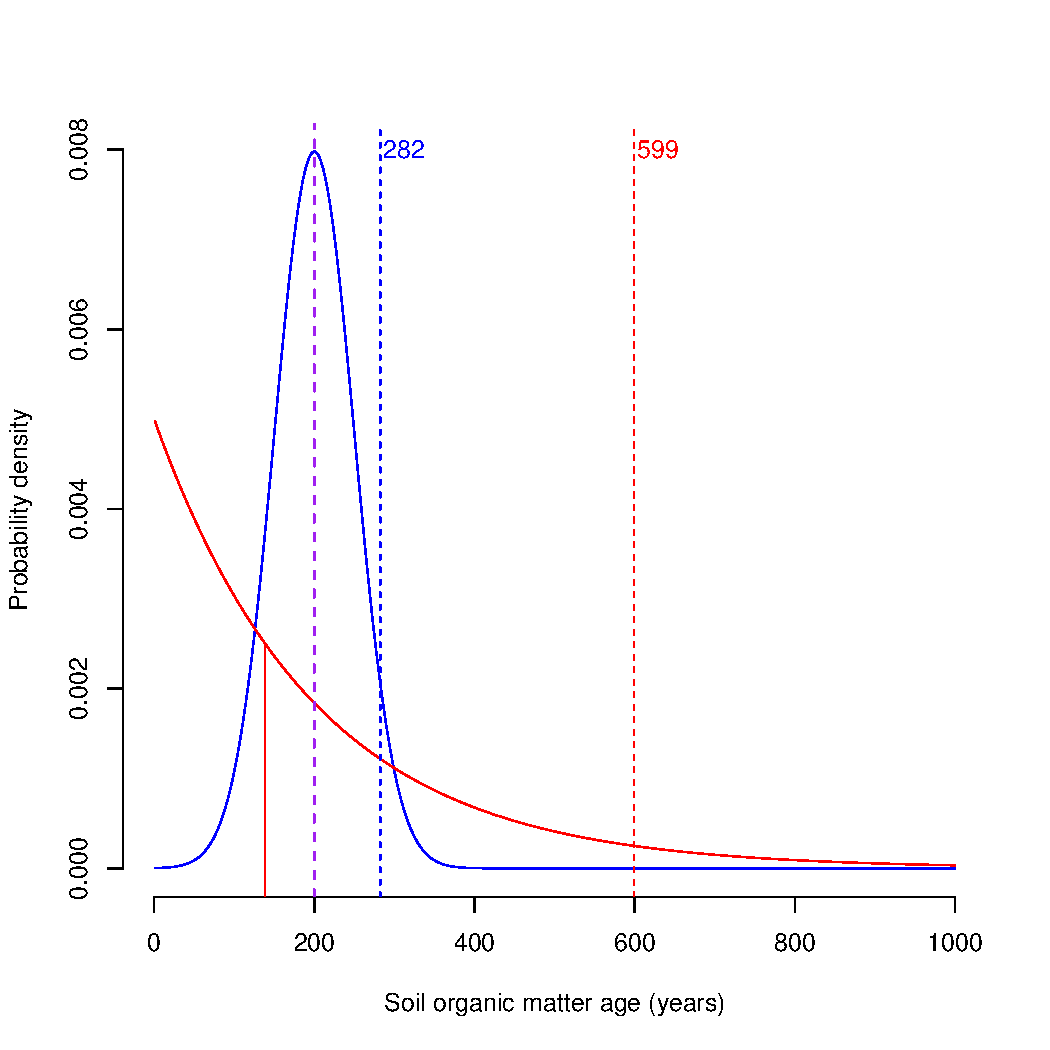
\includegraphics[scale=0.75]{Figures/example} % requires the graphicx package
   \caption{Soil organic matter age for two hypothetical soils with similar mean age, but with different density functions. In both cases, the mean age is 200 years (purple vertical line), but for the exponentially distributed soil the 95\% quantile $Q_{95} = 599$ years, while for the normally distributed soil (blue line) $Q_{95} = 282$ years. In asymmetric distributions with long tails such as the exponential or the phase-type, the mean is more sensitive to the skewness than the median. In this example, the 50\% quantile $Q_{50} = 139$ years (vertical solid red line) for the exponential distribution.}
   \label{fig:example}
\end{figure}

%Fig 2
\begin{figure}[t]
   \centering
%   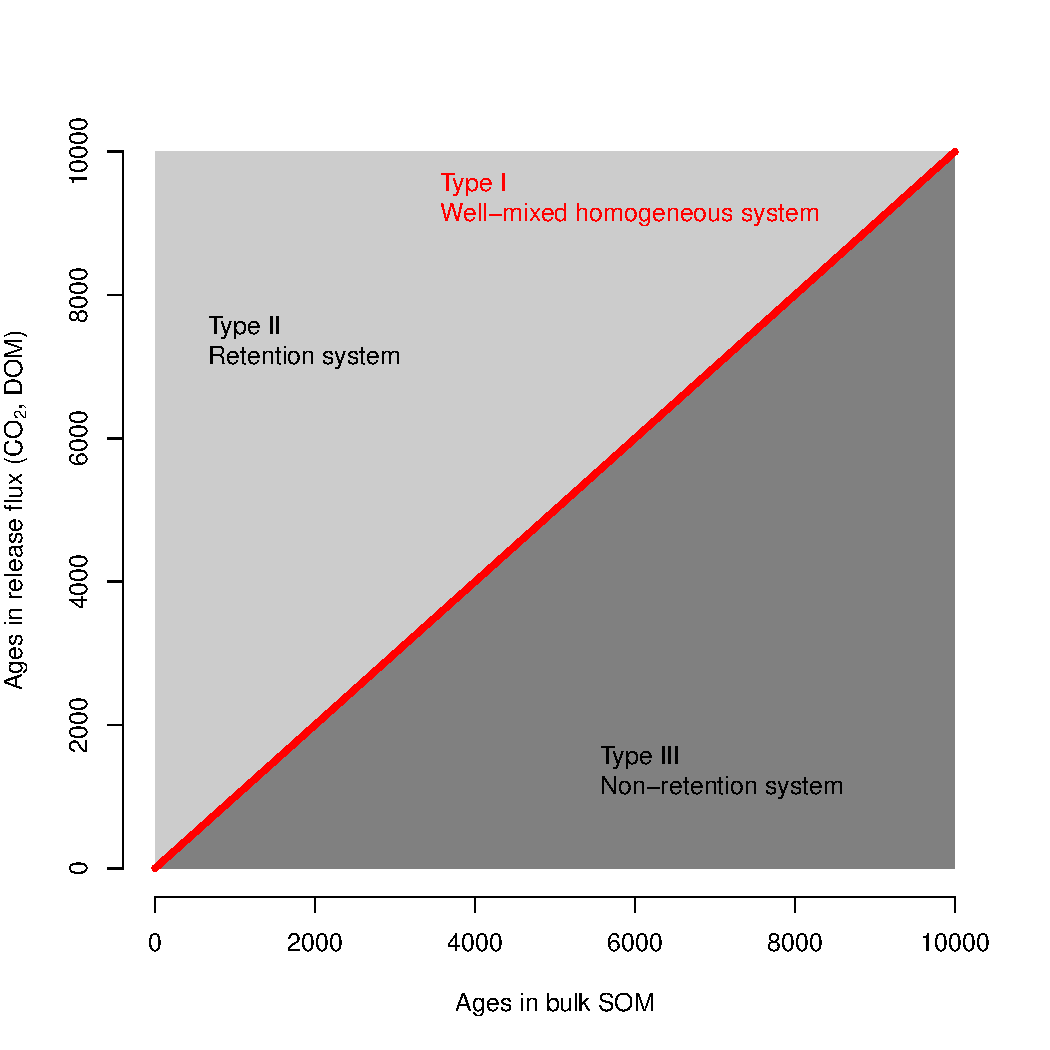
\includegraphics[scale=0.75]{Figures/systemTypes} % requires the graphicx package
   \caption{Possible relations between ages and transit times of organic matter in soils. Axes in arbitrary time units, e.g. days, months, years.}
   \label{fig:hypotheses}
\end{figure}

%Fig 3
\begin{figure}[t]
   \centering
%   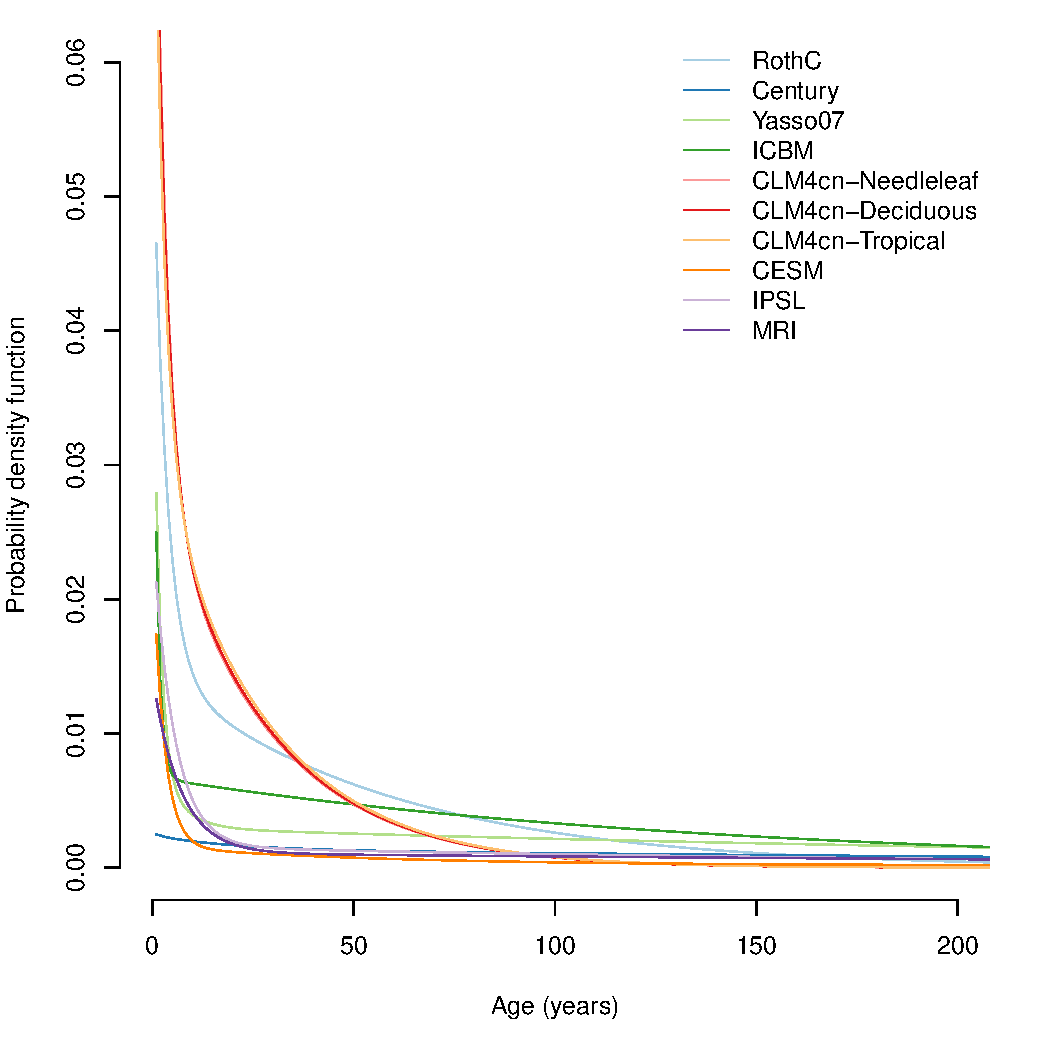
\includegraphics[scale=0.75]{Figures/modelsSA} % requires the graphicx package
   \caption{Age density distribution functions of soil organic carbon calculated for the models described in Table (\ref{tab:models}).}
   \label{fig:ageDensity}
\end{figure}

%Fig 4
\begin{figure}[t]
   \centering
%   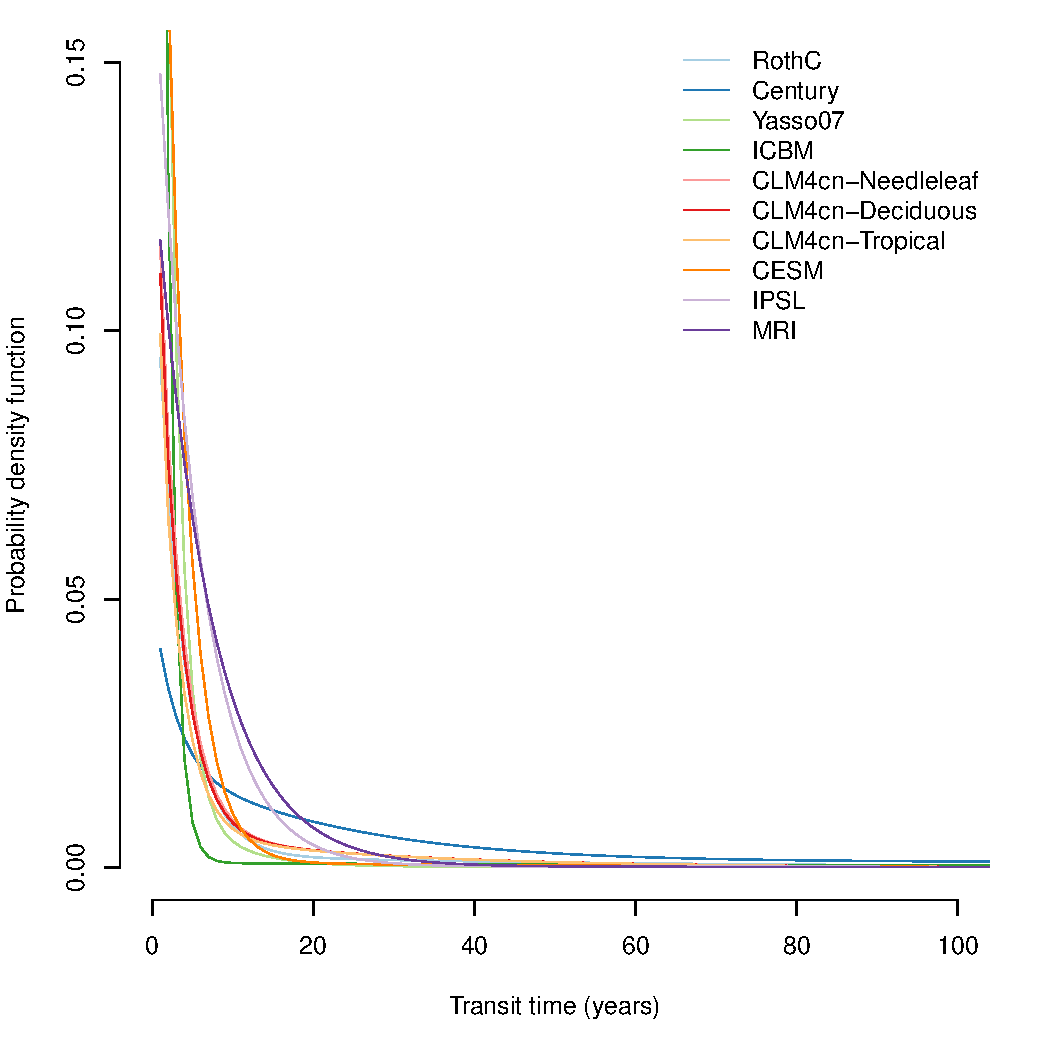
\includegraphics[scale=0.75]{Figures/modelsTT} % requires the graphicx package
   \caption{Transit time density distribution functions of soil organic carbon calculated for the models described in Table (\ref{tab:models}).}
   \label{fig:ttDensity}
\end{figure}

% Fig 5
\begin{figure}[t]
   \centering
%   \includegraphics[scale=0.75]{Figures/modelQ} % requires the graphicx package
   \caption{Sequence of quantiles, from 5 to 95\% by 5\% increments, for the age and transit time distributions of soil organic carbon calculated for the models of Table (\ref{tab:models}). Dashed line represents the 1:1 line. Notice that axes are in logarithmic scale.}
   \label{fig:quantiles}
\end{figure}

%Fig 6
\begin{figure}[htbp]
   \centering
%   \includegraphics[scale=0.8]{Figures/corrsattESMs} % requires the graphicx package
   \caption{Mean age and mean transit times of soil organic carbon predicted for each grid cell by the three versions of the reduced complexity Earth system models CESM, IPSL, and MRI, corrected by observations of radiocarbon in soil profiles as described in \citet{He2016}. Dashed line represents the 1:1 line. }
   \label{fig:sattESMs}
\end{figure}

%Fig 7
\begin{figure}[htbp]
   \centering
%   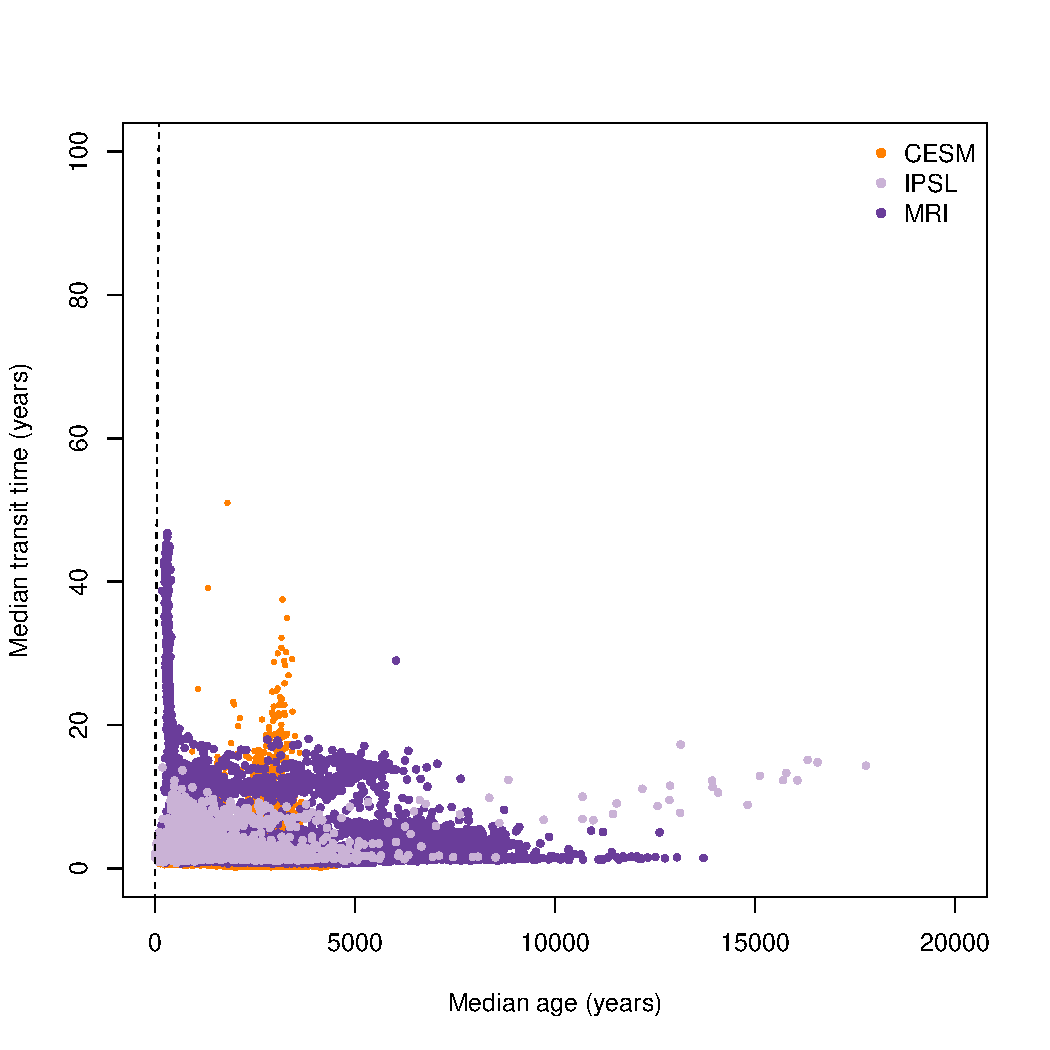
\includegraphics[scale=0.8]{Figures/corrQ50ESMs} % requires the graphicx package
   \caption{Median age and median transit times ($Q_{50}$) of soil organic carbon predicted for each grid cell by the three versions of the reduced complexity Earth system models CESM, IPSL, and MRI, corrected by observations of radiocarbon in soil profiles as described in \citet{He2016}. Dashed line represents the 1:1 line. }
   \label{fig:Q50ESMs}
\end{figure}


\clearpage

\section*{Appendix}
\subsection*{Matrix representation of analyzed models}
Each model was represented as a compartmental system of the form of equation (\ref{lam}). Below, we present the specific form of the matrix $\mathbf{B}$ and the vector ${\bm u}$  with the parameter values used for each model. 

\subsubsection*{RothC}
\begin{equation}
\mathbf{B} =
%% latex table generated in R 3.3.3 by xtable 1.8-2 package
% Sat Feb 17 10:47:45 2018
\begin{pmatrix}{}
  -10.00 & 0.00 & 0.00 & 0.00 \\ 
  0.00 & -0.30 & 0.00 & 0.00 \\ 
  1.02 & 0.03 & -0.59 & 0.00 \\ 
  1.20 & 0.04 & 0.08 & -0.02 \\ 
  \end{pmatrix}
,
% latex table generated in R 3.3.3 by xtable 1.8-2 package
% Sat Feb 17 10:47:45 2018
\begin{pmatrix}{}
  -10.00 & 0.00 & 0.00 & 0.00 \\ 
  0.00 & -0.30 & 0.00 & 0.00 \\ 
  1.02 & 0.03 & -0.59 & 0.00 \\ 
  1.20 & 0.04 & 0.08 & -0.02 \\ 
  \end{pmatrix}
\quad {\bm u} =
%% latex table generated in R 3.3.3 by xtable 1.8-2 package
% Sat Feb 17 11:06:23 2018
\begin{pmatrix}{}
  1.00 \\ 
  0.70 \\ 
  0.00 \\ 
  0.00 \\ 
  \end{pmatrix}
.
% latex table generated in R 3.3.3 by xtable 1.8-2 package
% Sat Feb 17 11:06:23 2018
\begin{pmatrix}{}
  1.00 \\ 
  0.70 \\ 
  0.00 \\ 
  0.00 \\ 
  \end{pmatrix}
\end{equation}

\subsubsection*{Century}
\begin{equation}
\mathbf{B} =
%% latex table generated in R 3.3.3 by xtable 1.8-2 package
% Sat Feb 17 11:26:32 2018
\begin{pmatrix}{}
  -0.069637 & 0.000000 & 0.000000 & 0.000000 & 0.000000 \\ 
  0.000000 & -0.350000 & 0.000000 & 0.000000 & 0.000000 \\ 
  0.031337 & 0.192500 & -0.071750 & 0.001596 & 0.000058 \\ 
  0.020891 & 0.000000 & 0.042189 & -0.003800 & 0.000000 \\ 
  0.000000 & 0.000000 & 0.000287 & 0.000114 & -0.000130 \\ 
  \end{pmatrix}
,
% latex table generated in R 3.3.3 by xtable 1.8-2 package
% Sat Feb 17 11:26:32 2018
\begin{pmatrix}{}
  -0.069637 & 0.000000 & 0.000000 & 0.000000 & 0.000000 \\ 
  0.000000 & -0.350000 & 0.000000 & 0.000000 & 0.000000 \\ 
  0.031337 & 0.192500 & -0.071750 & 0.001596 & 0.000058 \\ 
  0.020891 & 0.000000 & 0.042189 & -0.003800 & 0.000000 \\ 
  0.000000 & 0.000000 & 0.000287 & 0.000114 & -0.000130 \\ 
  \end{pmatrix}
\quad {\bm u} =
%% latex table generated in R 3.3.3 by xtable 1.8-2 package
% Sat Feb 17 11:29:16 2018
\begin{pmatrix}{}
  0.08 \\ 
  0.02 \\ 
  0.00 \\ 
  0.00 \\ 
  0.00 \\ 
  \end{pmatrix}
.
% latex table generated in R 3.3.3 by xtable 1.8-2 package
% Sat Feb 17 11:29:16 2018
\begin{pmatrix}{}
  0.08 \\ 
  0.02 \\ 
  0.00 \\ 
  0.00 \\ 
  0.00 \\ 
  \end{pmatrix}
\end{equation}

\subsubsection*{Yasso07}
\begin{equation}
\mathbf{B} =
%% latex table generated in R 3.3.3 by xtable 1.8-2 package
% Sat Feb 17 11:34:39 2018
\begin{pmatrix}{}
  -0.6600 & 1.3760 & 0.0035 & 0.2046 & 0.0000 \\ 
  0.2244 & -4.3000 & 0.0000 & 0.0000 & 0.0000 \\ 
  0.0231 & 0.0215 & -0.3500 & 0.0022 & 0.0000 \\ 
  0.0003 & 0.1290 & 0.3220 & -0.2200 & 0.0000 \\ 
  0.0264 & 0.1720 & 0.0140 & 0.0088 & -0.0033 \\ 
  \end{pmatrix}
,
% latex table generated in R 3.3.3 by xtable 1.8-2 package
% Sat Feb 17 11:34:39 2018
\begin{pmatrix}{}
  -0.6600 & 1.3760 & 0.0035 & 0.2046 & 0.0000 \\ 
  0.2244 & -4.3000 & 0.0000 & 0.0000 & 0.0000 \\ 
  0.0231 & 0.0215 & -0.3500 & 0.0022 & 0.0000 \\ 
  0.0003 & 0.1290 & 0.3220 & -0.2200 & 0.0000 \\ 
  0.0264 & 0.1720 & 0.0140 & 0.0088 & -0.0033 \\ 
  \end{pmatrix}
\quad {\bm u} =
%% latex table generated in R 3.3.3 by xtable 1.8-2 package
% Sat Feb 17 11:29:10 2018
\begin{pmatrix}{}
  10.00 \\ 
  0.00 \\ 
  0.00 \\ 
  0.00 \\ 
  0.00 \\ 
  \end{pmatrix}
.
% latex table generated in R 3.3.3 by xtable 1.8-2 package
% Sat Feb 17 11:29:10 2018
\begin{pmatrix}{}
  10.00 \\ 
  0.00 \\ 
  0.00 \\ 
  0.00 \\ 
  0.00 \\ 
  \end{pmatrix}
\end{equation}

\subsubsection*{ICBM}
\begin{equation}
\mathbf{B} =
%% latex table generated in R 3.3.3 by xtable 1.8-2 package
% Sat Feb 17 11:34:32 2018
\begin{pmatrix}{}
  -0.9360 & 0.0000 \\ 
  0.1170 & -0.0071 \\ 
  \end{pmatrix}
,
% latex table generated in R 3.3.3 by xtable 1.8-2 package
% Sat Feb 17 11:34:32 2018
\begin{pmatrix}{}
  -0.9360 & 0.0000 \\ 
  0.1170 & -0.0071 \\ 
  \end{pmatrix}
\quad {\bm u} =
%% latex table generated in R 3.3.3 by xtable 1.8-2 package
% Sat Feb 17 11:34:56 2018
\begin{pmatrix}{}
  0.06 \\ 
  0.00 \\ 
  \end{pmatrix}
.
% latex table generated in R 3.3.3 by xtable 1.8-2 package
% Sat Feb 17 11:34:56 2018
\begin{pmatrix}{}
  0.06 \\ 
  0.00 \\ 
  \end{pmatrix}
\end{equation}

\subsubsection*{CLM4cn}
This model contains one single $\mathbf{B}$ matrix for all plant functional types (PFTs):
\begin{equation}
\mathbf{B} =
%% latex table generated in R 3.3.3 by xtable 1.8-2 package
% Sat Feb 17 11:48:29 2018
\begin{pmatrix}{}
  -434.0000 & 0.0000 & 0.0000 & 0.0000 & 0.0000 & 0.0000 & 0.0000 & 0.0000 \\ 
  0.0000 & -26.4700 & 0.0000 & 0.2776 & 0.0000 & 0.0000 & 0.0000 & 0.0000 \\ 
  0.0000 & 0.0000 & -5.1450 & 0.0876 & 0.0000 & 0.0000 & 0.0000 & 0.0000 \\ 
  0.0000 & 0.0000 & 0.0000 & -0.3652 & 0.0000 & 0.0000 & 0.0000 & 0.0000 \\ 
  264.7400 & 0.0000 & 0.0000 & 0.0000 & -26.4700 & 0.0000 & 0.0000 & 0.0000 \\ 
  0.0000 & 11.9115 & 0.0000 & 0.0000 & 19.0584 & -5.1450 & 0.0000 & 0.0000 \\ 
  0.0000 & 0.0000 & 3.6529 & 0.0000 & 0.0000 & 2.7783 & -0.5114 & 0.0000 \\ 
  0.0000 & 0.0000 & 0.0000 & 0.0000 & 0.0000 & 0.0000 & 0.2301 & -0.0365 \\ 
  \end{pmatrix}
.
% latex table generated in R 3.3.3 by xtable 1.8-2 package
% Sat Feb 17 11:48:29 2018
\begin{pmatrix}{}
  -434.0000 & 0.0000 & 0.0000 & 0.0000 & 0.0000 & 0.0000 & 0.0000 & 0.0000 \\ 
  0.0000 & -26.4700 & 0.0000 & 0.2776 & 0.0000 & 0.0000 & 0.0000 & 0.0000 \\ 
  0.0000 & 0.0000 & -5.1450 & 0.0876 & 0.0000 & 0.0000 & 0.0000 & 0.0000 \\ 
  0.0000 & 0.0000 & 0.0000 & -0.3652 & 0.0000 & 0.0000 & 0.0000 & 0.0000 \\ 
  264.7400 & 0.0000 & 0.0000 & 0.0000 & -26.4700 & 0.0000 & 0.0000 & 0.0000 \\ 
  0.0000 & 11.9115 & 0.0000 & 0.0000 & 19.0584 & -5.1450 & 0.0000 & 0.0000 \\ 
  0.0000 & 0.0000 & 3.6529 & 0.0000 & 0.0000 & 2.7783 & -0.5114 & 0.0000 \\ 
  0.0000 & 0.0000 & 0.0000 & 0.0000 & 0.0000 & 0.0000 & 0.2301 & -0.0365 \\ 
  \end{pmatrix}
\end{equation}

For the needleleaf, deciduous, and tropical PFTs, the vector ${\bm u}$ is given by, respectively
\begin{equation}
{\bm u} =
%% latex table generated in R 3.3.3 by xtable 1.8-2 package
% Sat Feb 17 11:49:30 2018
\begin{pmatrix}{}
  95.75 \\ 
  191.50 \\ 
  95.75 \\ 
  200.00 \\ 
  0.00 \\ 
  0.00 \\ 
  0.00 \\ 
  0.00 \\ 
  \end{pmatrix}
, 
% latex table generated in R 3.3.3 by xtable 1.8-2 package
% Sat Feb 17 11:49:30 2018
\begin{pmatrix}{}
  95.75 \\ 
  191.50 \\ 
  95.75 \\ 
  200.00 \\ 
  0.00 \\ 
  0.00 \\ 
  0.00 \\ 
  0.00 \\ 
  \end{pmatrix}
\quad {\bm u}=
%% latex table generated in R 3.3.3 by xtable 1.8-2 package
% Sat Feb 17 11:49:30 2018
\begin{pmatrix}{}
  105.50 \\ 
  211.00 \\ 
  105.50 \\ 
  180.00 \\ 
  0.00 \\ 
  0.00 \\ 
  0.00 \\ 
  0.00 \\ 
  \end{pmatrix}
, 
% latex table generated in R 3.3.3 by xtable 1.8-2 package
% Sat Feb 17 11:49:30 2018
\begin{pmatrix}{}
  105.50 \\ 
  211.00 \\ 
  105.50 \\ 
  180.00 \\ 
  0.00 \\ 
  0.00 \\ 
  0.00 \\ 
  0.00 \\ 
  \end{pmatrix}
\quad {\bm u}=
%% latex table generated in R 3.3.3 by xtable 1.8-2 package
% Sat Feb 17 11:49:30 2018
\begin{pmatrix}{}
  362.25 \\ 
  724.50 \\ 
  362.25 \\ 
  360.00 \\ 
  0.00 \\ 
  0.00 \\ 
  0.00 \\ 
  0.00 \\ 
  \end{pmatrix}
.
% latex table generated in R 3.3.3 by xtable 1.8-2 package
% Sat Feb 17 11:49:30 2018
\begin{pmatrix}{}
  362.25 \\ 
  724.50 \\ 
  362.25 \\ 
  360.00 \\ 
  0.00 \\ 
  0.00 \\ 
  0.00 \\ 
  0.00 \\ 
  \end{pmatrix}
\end{equation}

For the following reduced complexity models, the average of parameters across all grid cells is given by the following matrices

\subsubsection*{CESM}
\begin{equation}
\mathbf{B} =
%% latex table generated in R 3.3.3 by xtable 1.8-2 package
% Sat Feb 17 11:58:10 2018
\begin{pmatrix}{}
  -0.3595 & 0.0000 & 0.0000 \\ 
  0.0226 & -0.0180 & 0.0000 \\ 
  0.0000 & 0.0020 & -0.0002 \\ 
  \end{pmatrix}
,
% latex table generated in R 3.3.3 by xtable 1.8-2 package
% Sat Feb 17 11:58:10 2018
\begin{pmatrix}{}
  -0.3595 & 0.0000 & 0.0000 \\ 
  0.0226 & -0.0180 & 0.0000 \\ 
  0.0000 & 0.0020 & -0.0002 \\ 
  \end{pmatrix}
\quad {\bm u} =
%% latex table generated in R 3.3.3 by xtable 1.8-2 package
% Sat Feb 17 11:58:10 2018
\begin{pmatrix}{}
  0.31 \\ 
  0.00 \\ 
  0.00 \\ 
  \end{pmatrix}
.
% latex table generated in R 3.3.3 by xtable 1.8-2 package
% Sat Feb 17 11:58:10 2018
\begin{pmatrix}{}
  0.31 \\ 
  0.00 \\ 
  0.00 \\ 
  \end{pmatrix}
\end{equation}

\subsubsection*{IPSL}
\begin{equation}
\mathbf{B} =
%% latex table generated in R 3.3.3 by xtable 1.8-2 package
% Sat Feb 17 12:02:09 2018
\begin{pmatrix}{}
  -0.19021 & 0.00000 & 0.00000 \\ 
  0.01160 & -0.00459 & 0.00000 \\ 
  0.00000 & 0.00009 & -0.00006 \\ 
  \end{pmatrix}
,
% latex table generated in R 3.3.3 by xtable 1.8-2 package
% Sat Feb 17 12:02:09 2018
\begin{pmatrix}{}
  -0.19021 & 0.00000 & 0.00000 \\ 
  0.01160 & -0.00459 & 0.00000 \\ 
  0.00000 & 0.00009 & -0.00006 \\ 
  \end{pmatrix}
\quad {\bm u} =
%% latex table generated in R 3.3.3 by xtable 1.8-2 package
% Sat Feb 17 12:02:22 2018
\begin{pmatrix}{}
  0.63 \\ 
  0.00 \\ 
  0.00 \\ 
  \end{pmatrix}
.
% latex table generated in R 3.3.3 by xtable 1.8-2 package
% Sat Feb 17 12:02:22 2018
\begin{pmatrix}{}
  0.63 \\ 
  0.00 \\ 
  0.00 \\ 
  \end{pmatrix}
\end{equation}

\subsubsection*{MRI}
\begin{equation}
\mathbf{B} =
%% latex table generated in R 3.3.3 by xtable 1.8-2 package
% Sat Feb 17 12:04:52 2018
\begin{pmatrix}{}
  -0.14629 & 0.00000 & 0.00000 \\ 
  0.01110 & -0.00288 & 0.00000 \\ 
  0.00000 & 0.00010 & -0.00007 \\ 
  \end{pmatrix}
,
% latex table generated in R 3.3.3 by xtable 1.8-2 package
% Sat Feb 17 12:04:52 2018
\begin{pmatrix}{}
  -0.14629 & 0.00000 & 0.00000 \\ 
  0.01110 & -0.00288 & 0.00000 \\ 
  0.00000 & 0.00010 & -0.00007 \\ 
  \end{pmatrix}
\quad {\bm u} =
%% latex table generated in R 3.3.3 by xtable 1.8-2 package
% Sat Feb 17 12:05:08 2018
\begin{pmatrix}{}
  0.76 \\ 
  0.00 \\ 
  0.00 \\ 
  \end{pmatrix}
.
% latex table generated in R 3.3.3 by xtable 1.8-2 package
% Sat Feb 17 12:05:08 2018
\begin{pmatrix}{}
  0.76 \\ 
  0.00 \\ 
  0.00 \\ 
  \end{pmatrix}
\end{equation}

%\newpage
%
%\subsection*{Relationship between mean age and mean transit time}
%Consider the linear autonomous compartmental system given by
%\begin{equation}
%\bm{\dot{x}} = \bm{u} + \mathbf{B} \cdot \bm{x},
%\end{equation}
%where $\bm{x}$ is a vector of carbon stocks, $\bm{u}$ is a vector of inputs to the system, and $\mathbf{B}$ is a compartmental matrix. At steady-state, the solution of the system is given by
%\begin{equation}
%\bm{x}^* = - \mathbf{B}^{-1} \cdot \bm{u}
%\end{equation}
%
%\subsubsection*{Mean age equal to mean transit time}
%To analyze the relationship between age and transit time, 
%we begin by considering the case where the mean age $\mathbb{E} (A)$ is equal to the mean transit time $\mathbb{E} (T)$, which implies
%
%\begin{align}
%\mathbb{E} (A) &= \mathbb{E} (T), \notag \\
%-\mathbf{1}^{T} \cdot \mathbf{B}^{-1} \frac{\bm{x}^*}{|| \bm{x}^* ||} &= -\mathbf{1}^{T} \cdot \mathbf{B}^{-1} \frac{\bm{u}}{|| \bm{u} ||}, \notag \\
% \frac{\bm{x}^*}{|| \bm{x}^* ||} &= \frac{\bm{u}}{|| \bm{u} ||}. \notag
%\end{align}
%
%For this equality to hold, the relative proportion of the input vector must be equal to the relative proportion of stocks at steady-state. This can only occur in two different cases, when the system is of dimension 1 (one single pool at steady-state), or when the vector $\bm{u}$ is proportional to one of the eigenvalues of $\mathbf{B}^{-1}$ as we will see in the next paragraph. 
%
%Recall that any vector $\bm{v}$ that follows the property $\mathbf{A} \bm{v} = \lambda \bm{v}$ is an eigenvector of the square matrix $\mathbf{A}$ with a corresponding eigenvalue $\lambda$. Now, from the identity above, we have
%
%\begin{equation}
%\bm{x}^* = \frac{|| \bm{x}^* ||}{|| \bm{u} ||} \cdot \bm{u} = \mathbb{E} (T) \cdot \bm{u} = - \mathbf{B}^{-1} \cdot \bm{u},
%\end{equation}
%therefore, if the mean age is equal to the mean transit time, the vector of inputs must be an eigenvector of the matrix $- \mathbf{B}^{-1}$, which is proportional to the eigenvalue characterized by the mean transit time. 
%
%\subsubsection*{Mean age higher than mean transit time}
%We will consider now the most common case when the mean age is different than the mean transit time. 



\end{document}  